\defChapterTarget[ImplementationIntegrationAndTestPlan]{Implementation, integration and test plan}
    \section{Implementation plan}
    SafeStreets system is composed by different subsystems:
    \begin{itemize}
        \item MobileApp
        \item WebServerApp
        \item AuhtorityUserWebApp
        \item ApplicationServer
        \item SafeStreets DBMS
    \end{itemize}   
    All SafeStreets subsystems need to be implemented, tested and integrated
    using a bottom-up approach. With a bottom-up strategy it's possible to
    develop lower level components first and then to reuse them in order to
    create higher level elements. Bottom-up approach also allows better testing
    of all the different components. It's important to show a visible
    application feature during all the steps of the development.\\
    There also are some external subsystems: 
    \begin{itemize}
        \item Municipality DBMS
        \item Google Maps
        \item Plate Recognizer
        \item Ghiro
    \end{itemize}   
    All the external subsystems, of course, are not implemented and tested
    because are develope by other people and they can be considered trustworthy.\\
    It's useful to create a list with all the features, their importance for the
    customer and their difficulty of Implementation in order to have a better
    estimation of the order and the time needed to meet clients requirements.
    \begin{table}[]
        \begin{tabular}{|l|l|l|}
            \hline
            \textbf{Feature} & \textbf{Importance for the customer}  & \textbf{Implementation difficulty}  \\ \hline
            SignUp and SignIn & Low  & Low  \\ \hline
            Signal a violation & High  & High  \\ \hline
            Manage previous reports & Medium  & Medium  \\ \hline
            Visualize unsafe areas & High & High  \\ \hline
            Manage Account Settings & High & Low  \\ \hline
            Violation Checking & High & High  \\ \hline
            Visualize Statistics & High & High  \\ \hline
        \end{tabular}
    \end{table}
    
    \section{Integration and testing}
    \begin{table}
        \begin{tabular}{|l|l|l|}
            \hline
            \textbf{Component} & \textbf{Implementation percentage} & \textbf{Comments}\\ \hline
            Manage Account settings & 90-95 & \begin{minipage}[t]{0.4\textwidth}This functionality is important
            for the user but we can see it as an extra accessory that does not
            affect the other features of the system, and for this reason the
            corresponding component 'AccountManager' can be implemented and
            tested later than the others.\\\end{minipage} \\\hline
            
        \end{tabular}
        
    \end{table}
        \subsection{Entry criteria}
        \subsection{Elements to be integrated}
        \subsection{Integration testing strategy}
        \subsection{Sequence of component/function integration}

        \subsubsection{Integration of frontend and backend}
            \begin{figure}[H]
                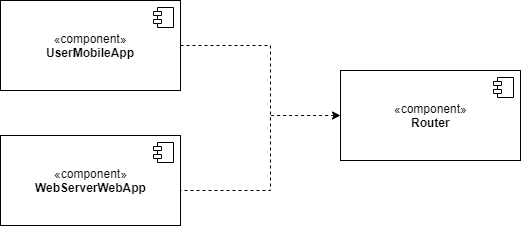
\includegraphics[scale=0.7]{dd/resources/images/Integration-Router.png}
                \caption{Router integration}        
            \end{figure}
            \begin{figure}[H]
                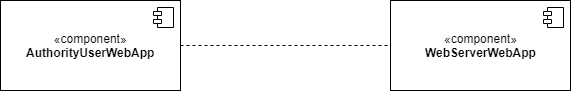
\includegraphics[scale=0.65]{dd/resources/images/Integration-Web.png}
                \caption{AuthorityUserWebApp-WebServerWebApp integration}        
            \end{figure}

        \subsubsection{External services integration}    
            \begin{figure}[H]
                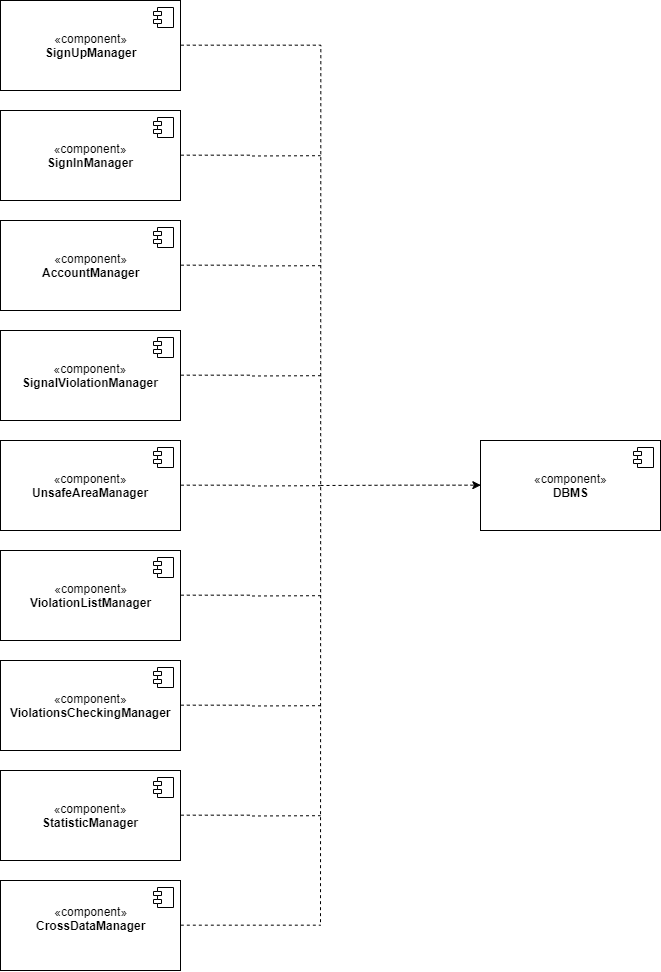
\includegraphics[scale=0.5]{dd/resources/images/Integration-DBMS.png}
                \caption{DBMS integration}        
            \end{figure}
            \begin{figure}[H]
                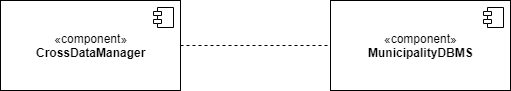
\includegraphics[scale=0.7]{dd/resources/images/Integration-MunicipalityDBMS.png}
                \caption{MunicipalityDBMS integration}        
            \end{figure}
            \begin{figure}[H]
                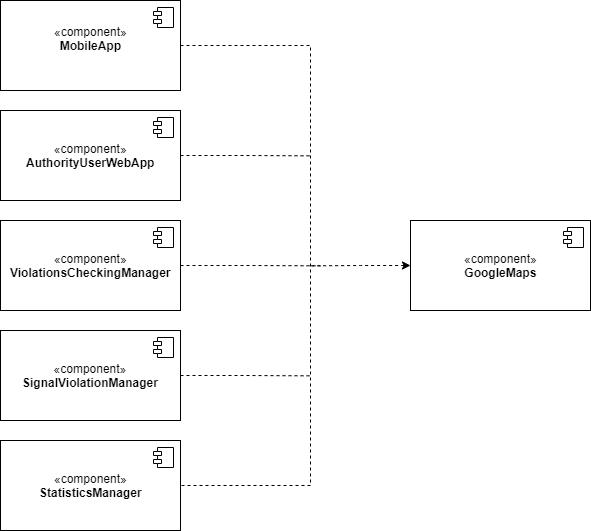
\includegraphics[scale=0.7]{dd/resources/images/Integration-GoogleMaps.png}
                \caption{Google Maps integration}        
            \end{figure}
            \begin{figure}[H]
                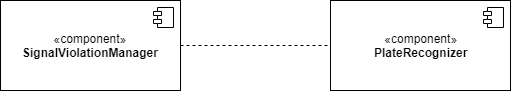
\includegraphics[scale=0.7]{dd/resources/images/Integration-PlateRecognizer.png}
                \caption{Plate Recognizer integration}        
            \end{figure}

        \subsubsection{External services integration}    
            \begin{figure}[H]
                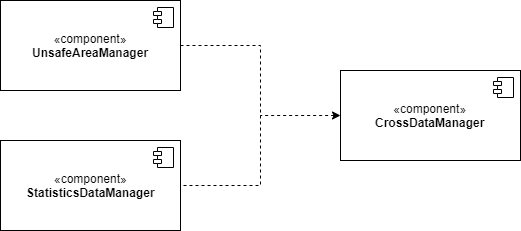
\includegraphics[scale=0.7]{dd/resources/images/Integration-CrossDataManager.png}
                \caption{CrossDataManager integration}        
            \end{figure}